\section{3.1.1.2 Conjugate Dynamics}
\begin{frame}{Conjugate Dynamics}
\begin{itemize}
    \item We start with the definition of conjugacy between dynamical systems ($(V, T_\sigma)$ is a dynamical system with state space $V$ and evolution $T_\sigma$).
    \item  Then, we go to the most basic structure, $V$ as a poset, and upgrade conjugacy to order conjugacy. 
    \item  This prepares for the later upgrade from dynamical system to ADP
\end{itemize}
\end{frame}
\begin{frame}{Definitions}
\begin{definition}
    We call a \textbf{discrete time dynamical system} is a pair $(V,S)$, where $V$ is any set, and $S$ is a self-map on $V$.
\end{definition}
\begin{definition}
    Two dynamical systems $(V, S)$ and $(\hat V, \hat S)$ are said to be \textbf{conjugate under $F$} if 
    $$
    \text{$F$ is a bijection from $V$ into $\hat V$ and $F\circ S = \hat S \circ F$ on V} 
    $$
    or we can write it as
    $$
    S = F^{-1} \circ \hat S \circ F
    $$
\end{definition}
\end{frame}

\begin{frame}{Proposition 3.1.2.}
    If $(V,S)$ and $(\hat V, \hat S)$ are conjugate, then
    \begin{enumerate}
        \item $S^n = F^{-1} \hat S^n F$ for all $n\in \mathbb{N}$
        \item $v$ is a fixed point of $S$ if and only if $Fv$ is a fixed point of $\hat S$
        \item $\hat v$ is fixed point of $\hat S$ if and only if $F^{-1}\hat v$ is a fixed point of $S$
        \item $v$ is the unique fixed point of $S$ in $V$ if and only if $Fv$ is the unique fixed point of $\hat S$ in $\hat V$.
    \end{enumerate}
    \begin{proof}
        Let $v$ be the unique fixed point of $S$, i.e., $Sv=v$. Hence, 
        $$
        F(v) = F(Sv) = \hat S(Fv)
        $$
        Hence, $F(v)$ is a fixed point of $\hat S$. Let $\hat w = F(w)$ be a fixed point $\hat S$, then by part 2, $w$ is the fixed point of $S$. Hence, $w=v$, and this implies $F(w)= F(v)$.
    \end{proof}
\end{frame}

\begin{frame}{Example 3.1.2}
   \begin{figure}
       \centering
       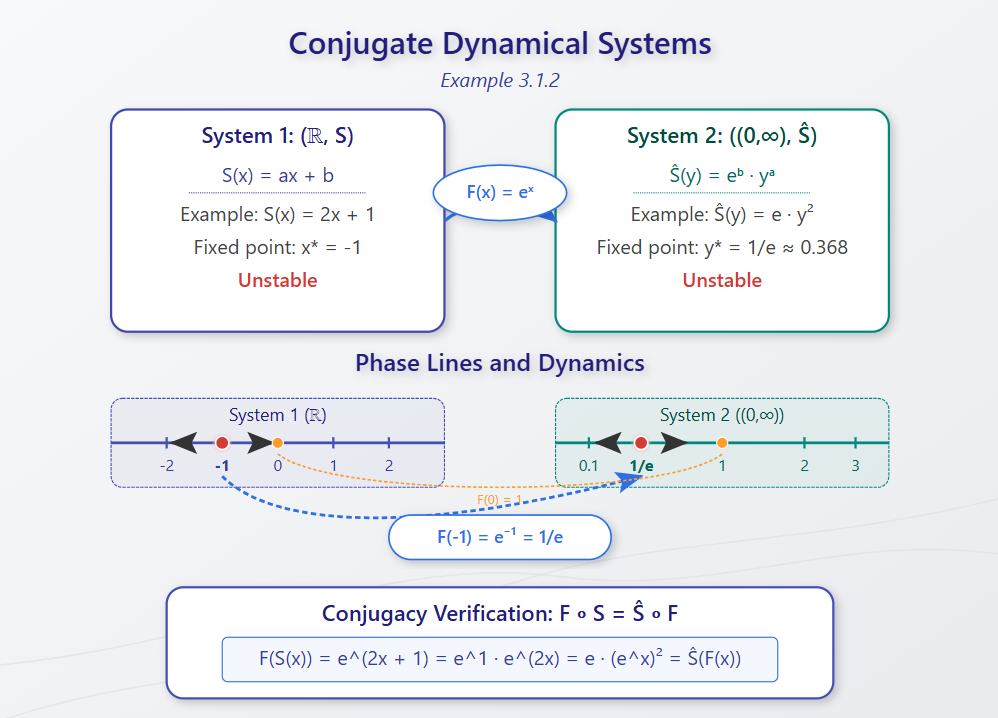
\includegraphics[width=0.68\linewidth]{image/Example 3.1.2.png}
       \caption{Caption}
       \label{fig:enter-label}
   \end{figure} 
\end{frame}

\begin{frame}{Order conjugacy}
\begin{definition}
    Consider two dynamical systems $(V,S)$ and $(\hat V, \hat S)$, where $V,\hat V$ are posets. We call these systems \textbf{order conjugate under $F$} if they are conjugate under $F$, and, $F$ is an order isomorphism.
\end{definition}
\end{frame}

\begin{frame}{Exercise 3.1.9.}
Prove that order conjugacy is an equivalence relation on the set of dynamical systems over partially ordered set.
\begin{proof}
    We denote $(V,S)\sim (\hat{V},\hat S)$ is they are order conjugate. We need to show this relation is reflexive, symmetric and transitive. 
    \begin{itemize}
        \item (Reflexivity) Let $F=Id$ which is a bijection. We have 
        $$
        F\circ S = S = S\circ F 
        $$
        Moreover, we have $F = F^{-1}$ is order preserving. Hence, 
        $$
        (V,S) \sim (V,S)
        $$
    \end{itemize}
\end{proof}
\end{frame}

\begin{frame}{Exercise 3.1.9 Continue}
\begin{proof}
        \begin{itemize}
        \item (Symmetry) Let $(V,S)\sim (\hat V,\hat S)$ under $F$. 
        \begin{itemize}
            \item $F$ is bijection implies $F^{-1}$ is bijection
            \item $F\circ S = \hat S\circ F\implies F^{-1} \circ \hat S = S\circ F^{-1}$ 
        \end{itemize}
        Hence, $(V,S)$ and $(\hat V,\hat S)$ are conjugate under $F^{-1}$.
        \begin{itemize}
            \item $F$ is order preserving with order preserving inverse implies $F^{-1}$ is order preserving with order preserving inverse
        \end{itemize}
        Hence, $F^{-1}$ is order isomorphism. Hence $(\hat V,\hat S)\sim (V,S)$
    \end{itemize}
\end{proof}
\end{frame}

\begin{frame}{Exercise 3.1.9 Continue}
\begin{proof}
    \begin{itemize}
        \item (Transitive) Let $(V_1, S_1)\sim (V_2,S_2)$ under $F$ and $(V_2,S_2)\sim (V_3, S_3)$ under $G$. 
        \begin{itemize}
            \item $F,G$ are bijective implies $H := (G\circ F)$ is bijective
            \item $F\circ S_1 = S_2\circ F, G\circ S_2 = S_3\circ G\implies  (G\circ F)\circ S_1 = G\circ S_2 \circ F = S_3\circ(G\circ F)$
        \end{itemize}
        Hence, $(V_1,S_1)$ and $(V_3,S_3)$ are conjugate under $H$.
        \begin{itemize}
            \item $F,G$ are order preserving with order perserving inverses
            \item $G\circ F$ are order preserving with order preserving inverses
        \end{itemize}
        Hence, $(V_1,S_1)\sim (V_3, S_3)$ under $(G\circ F)$.
    \end{itemize}
\end{proof}
    
\end{frame}

\begin{frame}{Lemma 3.1.3.}
If $(V,S)$ and $(\hat V,\hat S)$ are order conjugate under $F$, then $S$ is order stable on $V$ if and only if $\hat S$ is order stable on $\hat V$.
\begin{proof}
    $(\implies)$ Suppose $S$ is order stable on $V$. This implies
    \begin{itemize}
        \item[(S1)] $S$ has a unique fixed point $v^*\in V$
        \item[(S2)] $v\in V, v\precsim v^*\implies v\precsim Sv$ and $v\in V, v^*\precsim v\implies Sv\precsim v$
    \end{itemize}
    $(S1)$ implies $\hat S$ has a unique fixed point $\hat v^* : =F(v)\in \hat V$ by Proposition 3.1.2. Moreover we have
    \begin{itemize}
        \item For $\hat v:= F(v)\in \hat V, \hat v\le \hat v^*\underbrace{\implies}_{o.i.} v\precsim v^*\underbrace{\implies}_{S2} v\precsim Sv\underbrace{\implies}_{o.i.}Fv\le \underbrace{FSv = \hat S\hat v}_{conjugate}$
        
    \end{itemize}
    
    
\end{proof}
    
\end{frame}